% This is auto-generated file: do not edit!
% Exported from microMathematics Plus, version 2.15.6


Jetzt zeichnen wir eine Funktion, die
im Polarkoordinatensystem gegeben ist.
Jeder Punkt in diesem System wird vom
Abstand r zum Ursprung und dem Winkel
f von der x-Achse bestimmt.
\begin{center}\begin{tabular}{c} 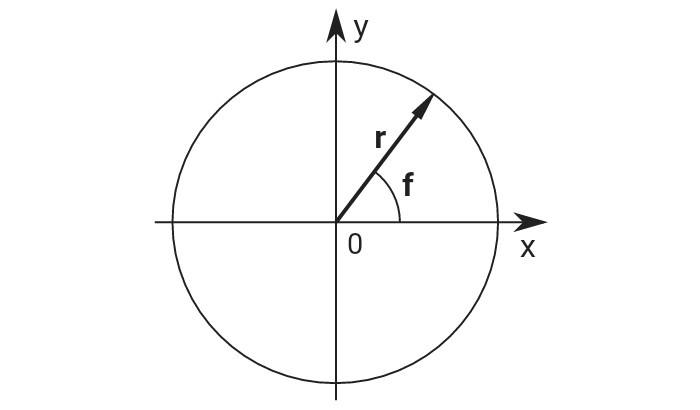
\includegraphics[resolution=320]{graphics/polar_plot_fig1.png} \end{tabular}\end{center}

Der Winkel f ist unsere unabhängige
Variable und wird folgendermaßen
angepasst:
\begin{center}\begin{tabular}{c}
  $f := \left[ 0.01,\, 0.05 \,..\, 300 \right]$
\end{tabular}\end{center}

Der Abstand r(f) ist unsere abhängige
Variable. Mittels des Paares f und r
können wir sie in die kartesischen
Koordinaten x und y umwandeln, indem
wir Sinus- und Kosinus-Funktionen
verwenden:
\begin{center}\begin{tabular}{cc}
  $x(r) := r \cdot cos \left( f\right) $ &
  $y(r) := r \cdot sin \left( f\right) $ \cr
\end{tabular}\end{center}

\subsection{Eine Schnecke}

Wir werden erste Polarfunktion in drei
Schritten definieren. Der erste
Ausdruck definiert ein ''Rad'':
\begin{center}\begin{tabular}{ccc}
  $A := 1.1$ &
  $B := 1.271$ &
  $q := 2$ \cr
\end{tabular}\end{center}
\begin{center}\begin{tabular}{c}
  $r1(f) := A + 2 \cdot {sin \left( B \cdot f\right) }^{q}$
\end{tabular}\end{center}

Um diese Funktion darzustellen, fügen
wir die Plot Box durch den ''Neu''
Button in der Menüleiste oder durch
''Funktionsgraph hinzufügen'' Button in
der Werkzeugleiste hinzu:
\begin{center}\begin{tabular}{c} 
\includegraphics[resolution=320]{graphics/polar_plot_fig2.png} \end{tabular}\end{center}

Anstelle von f und r benutzen wir die
zuvor definierten Regeln für
Umwandlungen von x und y, wobei rl(f)
als ein symbolisches Argument für
diese Regeln eingesetzt wird:
\begin{center}\begin{tabular}{c} 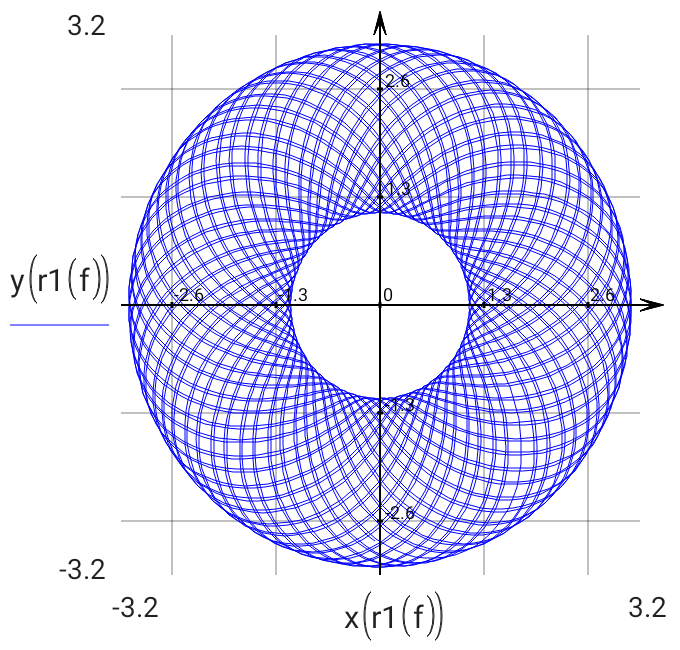
\includegraphics[resolution=320]{graphics/polar_plot_fig3.png} \end{tabular}\end{center}

Als nächstes können wir dieses Rad wie
folgt modifizieren:
\begin{center}\begin{tabular}{c}
  $r2(f) := A + 2 \cdot {sin \left( B \cdot f + 1 \cdot r1 \left( f\right) \right) }^{q}$
\end{tabular}\end{center}
\begin{center}\begin{tabular}{c} 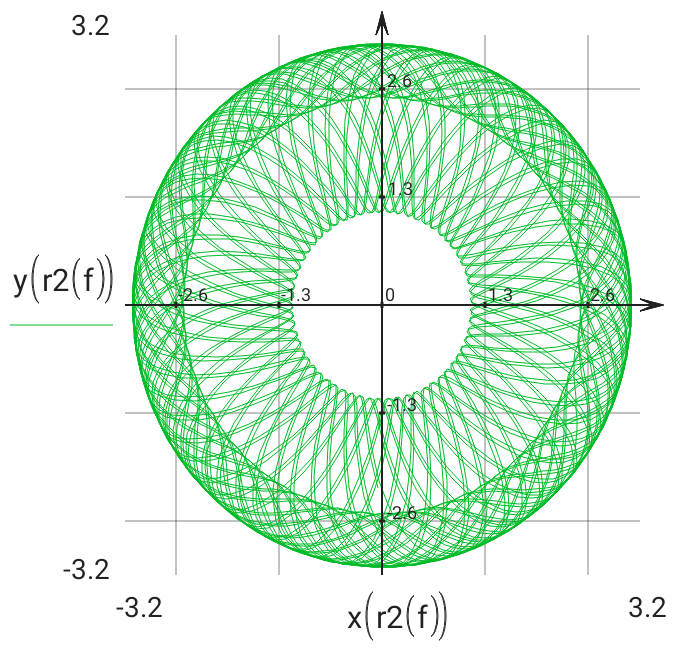
\includegraphics[resolution=320]{graphics/polar_plot_fig4.png} \end{tabular}\end{center}

Abschließend skalieren wir die letzte
Funktion r2(f), indem wir eine
Abrundung auf die nächstniedrigere
Ganzzahl verwenden, was wie eine
Stufenfunktion aussieht. Als Ergebnis
erhalten wir eine schöne Schnecke:
\begin{center}\begin{tabular}{c}
  $r(f) := r2 \left( f\right)  \cdot floor \left( f\right)  / 10$
\end{tabular}\end{center}
\begin{center}\begin{tabular}{c} 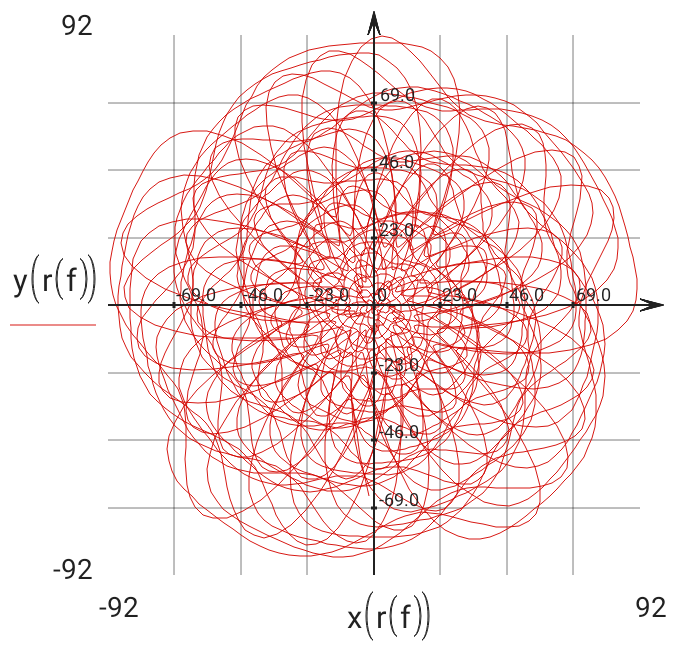
\includegraphics[resolution=320]{graphics/polar_plot_fig5.png} \end{tabular}\end{center}

\subsection{Japanischer Ahorn}

Japanischer Ahorn ist bekannt für die
schönen Formen und Farben seiner
Blätter. Solch ein Blatt kann
mathematisch beschrieben werden und
als Kurve im Polarkoordinatensystem
dargestellt werden:
\begin{center}\begin{tabular}{c}
  $f := \left[ 0.01,\, 0.02 \,..\, 100 \right]$
\end{tabular}\end{center}
\begin{center}\begin{tabular}{cc}
  $x(r) := r \cdot cos \left( f\right) $ &
  $y(r) := r \cdot sin \left( f\right) $ \cr
\end{tabular}\end{center}
\begin{center}\begin{tabular}{c}
  $s1(f) := \left( 1 + sin \left( f\right)  \right) \cdot \left( 1 - 0.9 \cdot  \left| sin \left( 4 \cdot f\right)  \right|  \right)$
\end{tabular}\end{center}
\begin{center}\begin{tabular}{c}
  $s2(f) := 0.9 + 0.05 \cdot cos \left( 200 \cdot f\right) $
\end{tabular}\end{center}
\begin{center}\begin{tabular}{c}
  $r(f) := floor \left( f\right)  \cdot s1 \left( f\right)  \cdot s2 \left( f\right)  + rnd \left( 2\right)  - 1$
\end{tabular}\end{center}
\begin{center}\begin{tabular}{c} 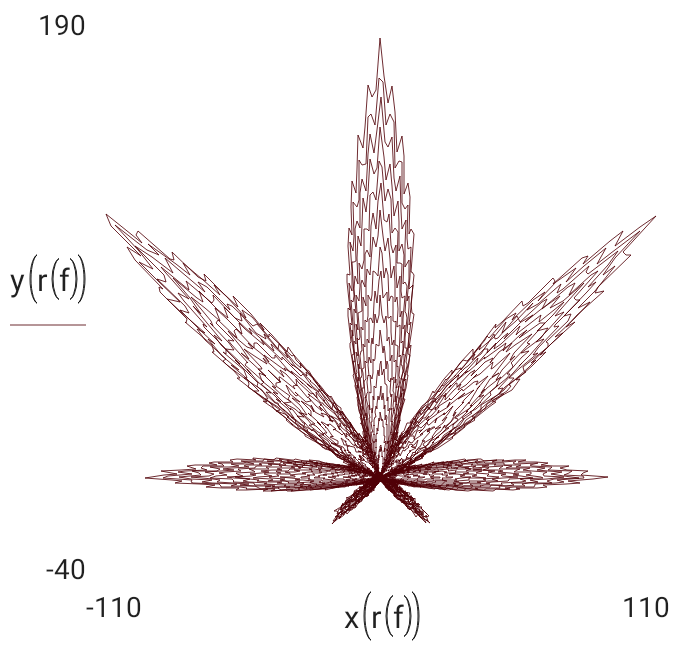
\includegraphics[resolution=320]{graphics/polar_plot_fig6.png} \end{tabular}\end{center}

http://en.wikipedia.org/wiki/Acer\_palmatum